%!TEX root = ../DA_MainDocument.tex

% ============================================================
% Listings-Stil fuer SQL und TypeScript
% ============================================================
\lstdefinelanguage{TypeScript}{
  keywords={const,let,var,function,return,async,await,if,else,throw,
            new,class,import,from,export,default,try,catch,true,false,
            null,undefined,void,string,number,boolean,Promise},
  sensitive=true,
  comment=[l]{//},
  morecomment=[s]{/*}{*/},
  morestring=[b]',
  morestring=[b]"
}

\lstdefinestyle{skyline-sql}{
  language=SQL,
  basicstyle=\footnotesize\ttfamily,
  keywordstyle=\bfseries,
  commentstyle=\color{gray}\itshape,
  stringstyle=\color{mydarkelectricblue},
  numbers=left,
  numberstyle=\tiny\color{gray},
  numbersep=8pt,
  frame=tb,
  rulecolor=\color{mydarkelectricblue},
  breaklines=true,
  showstringspaces=false,
  captionpos=b,
  morekeywords={UUID,BIGINT,TIMESTAMPTZ,BOOLEAN,REFERENCES,CASCADE,
                POLICY,USING,CHECK,ENABLE,ROW,LEVEL,SECURITY,
                gen_random_uuid,auth,uid,CREATE,TABLE,IF,NOT,EXISTS,
                PRIMARY,KEY,DEFAULT,ON,DELETE,SET,NULL,INDEX,
                DROP,ALTER}
}

\lstdefinestyle{skyline-ts}{
  language=TypeScript,
  basicstyle=\footnotesize\ttfamily,
  keywordstyle=\bfseries,
  commentstyle=\color{gray}\itshape,
  stringstyle=\color{mydarkelectricblue},
  numbers=left,
  numberstyle=\tiny\color{gray},
  numbersep=8pt,
  frame=tb,
  rulecolor=\color{mydarkelectricblue},
  breaklines=true,
  showstringspaces=false,
  captionpos=b
}

% ============================================================
\chapter{Implementierung: Zentrale \& sichere Datenverwaltung (JanOle)}\label{chapter:datenverwaltung}
% ============================================================

Dieses Kapitel beschreibt die konkrete Umsetzung der zentralen Datenverwaltung in Skyline.
Die theoretischen Grundlagen (Single Source of Truth, Sicherheitskonzept, Anforderungen)
werden in Kapitel~3 behandelt.

% ============================================================
\section{Implementierung in Skyline}
% ============================================================

Die zentrale Datenverwaltung in Skyline basiert auf Supabase Postgres als relationalem Kern
und Supabase Storage für dateibasierte Inhalte \cite{supabaseStorage}.
Im fachlichen Zentrum steht die Flugentität: Jeder Flug bildet einen konkreten Reisekontext,
an den Notizen, Checklisten und Dokumente angehängt werden.
Dadurch entsteht in Skyline kein loses Nebeneinander verschiedener Feature-Daten, sondern ein
zusammenhängendes Datenmodell, in dem jede Zusatzinformation eindeutig einem Flug zugeordnet ist.

Die Kernoperationen (Create, Read, Update, Delete) werden nicht direkt in den UI-Screens
implementiert, sondern über einen Service-Layer gekapselt (\texttt{services/supabase.ts},
\texttt{services/documentService.ts}).
Sicherheitsseitig wird Row-Level Security (RLS) auf Tabellenebene eingesetzt, sodass
Zugriffe bereits innerhalb der Datenbank an den authentifizierten Benutzerkontext gebunden sind.
Für den Teamkontext wurde das Modell migrationsbasiert erweitert: Über \texttt{company\_id}
können persönliche Flüge und Firmenflüge getrennt modelliert werden.
Mit \texttt{departure\_at} und \texttt{arrival\_at} wurden zeitbezogene Felder eingeführt,
die für Live-Progress auf der Karte sowie zeitbasierte Erinnerungslogik genutzt werden.

\begin{figure}[htbp]
  \centering
  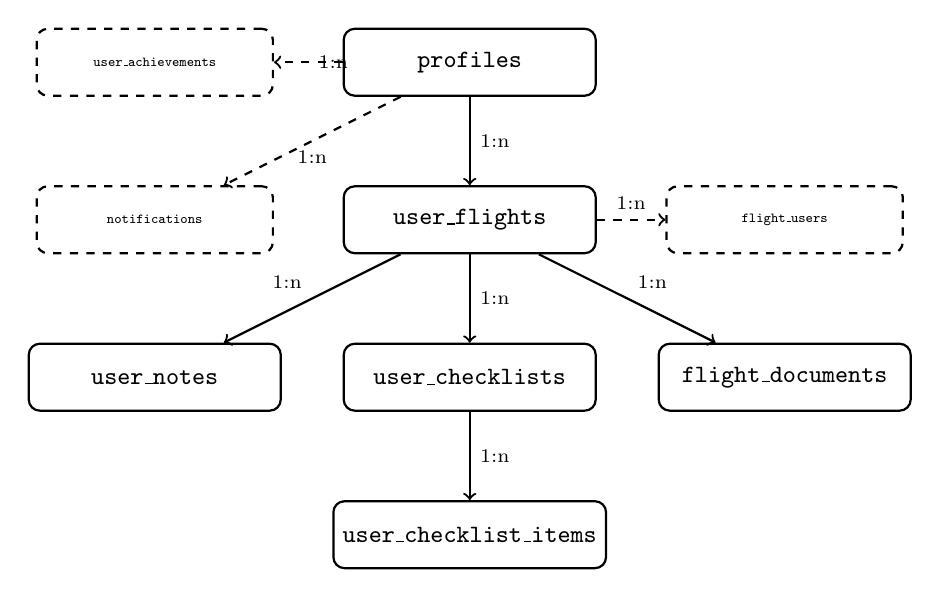
\begin{tikzpicture}[
    x=1cm, y=1cm,
    entity/.style={draw, rounded corners, thick, minimum width=3.2cm,
                   minimum height=0.85cm, align=center, font=\small\ttfamily},
    side/.style={draw, rounded corners, thick, minimum width=3.0cm,
                 minimum height=0.85cm, align=center, font=\tiny\ttfamily,
                 dashed},
    arr/.style={->, thick},
    sarr/.style={->, thick, dashed}
  ]
    \node[entity] (profiles)   at (0,0)    {profiles};
    \node[entity] (flights)    at (0,-2)   {user\_flights};
    \node[entity] (notes)      at (-4,-4)  {user\_notes};
    \node[entity] (checklists) at (0,-4)   {user\_checklists};
    \node[entity] (items)      at (0,-6)   {user\_checklist\_items};
    \node[entity] (documents)  at (4,-4)   {flight\_documents};
    \node[side]   (fusers)     at (4,-2)   {flight\_users};
    \node[side]   (notif)      at (-4,-2)  {notifications};
    \node[side]   (ach)        at (-4,0)   {user\_achievements};

    \draw[arr]  (profiles)   -- node[right, font=\scriptsize]{1:n} (flights);
    \draw[arr]  (flights)    -- node[above left, font=\scriptsize]{1:n} (notes);
    \draw[arr]  (flights)    -- node[right, font=\scriptsize]{1:n} (checklists);
    \draw[arr]  (checklists) -- node[right, font=\scriptsize]{1:n} (items);
    \draw[arr]  (flights)    -- node[above right, font=\scriptsize]{1:n} (documents);
    \draw[sarr] (flights)    -- node[above, font=\scriptsize]{1:n} (fusers);
    \draw[sarr] (profiles)   -- node[below, font=\scriptsize]{1:n} (notif);
    \draw[sarr] (profiles)   -- node[right, font=\scriptsize]{1:n} (ach);
  \end{tikzpicture}
  \caption{Zentrales Datenmodell in Skyline (vereinfachte ER-Darstellung;
           gestrichelt: ergänzende Feature-Tabellen)}
  \label{fig:datenmodell_skyline}
\end{figure}

% ============================================================
\subsection{Datenmodell \& Tabellenstruktur}
% ============================================================

Das relationale Kernmodell von Skyline besteht aus sechs operativen Tabellen und
einer zentralen Stammdatentabelle.
Im Folgenden werden alle Tabellen mit ihrer Struktur, ihren Constraints und
ihrer Rolle im Gesamtmodell beschrieben.

% ----------------------------------------------------------
\subsubsection*{Tabelle \texttt{profiles}}
% ----------------------------------------------------------

\texttt{profiles} bildet den nutzerbezogenen Einstiegspunkt.
Die Tabelle ist direkt mit dem internen Supabase-Auth-Kontext verknüpft:
\texttt{id} ist kein eigenständiger UUID-Wert, sondern ein Foreign Key auf
\texttt{auth.users(id)} -- das heißt, jeder Supabase-Nutzeraccount besitzt
genau einen Profilsatz.

Die Verknüpfung wird automatisch über einen Datenbank-Trigger hergestellt.
Listing~\ref{lst:profiles_trigger} zeigt Funktion und Trigger, die bei jeder
Neuregistrierung ausgeführt werden:

\begin{lstlisting}[style=skyline-sql,
  caption={Automatische Profilanlage via Trigger (complete\_working\_schema.sql)},
  label={lst:profiles_trigger}]
CREATE OR REPLACE FUNCTION public.handle_new_user()
RETURNS TRIGGER AS $$
BEGIN
  INSERT INTO public.profiles (id, full_name, avatar_url)
  VALUES (
    NEW.id,
    COALESCE(NEW.raw_user_meta_data->>'name', NEW.email),
    NEW.raw_user_meta_data->>'avatar_url'
  )
  ON CONFLICT (id) DO NOTHING;
  RETURN NEW;
END;
$$ LANGUAGE plpgsql SECURITY DEFINER;

CREATE TRIGGER on_auth_user_created
  AFTER INSERT ON auth.users
  FOR EACH ROW EXECUTE FUNCTION public.handle_new_user();
\end{lstlisting}

\begin{table}[htbp]
  \centering
  \caption{Felder der Tabelle \texttt{profiles}}
  \label{tab:profiles_felder}
  \begin{tabularx}{\textwidth}{l l X}
    \toprule
    \textbf{Feld} & \textbf{Typ} & \textbf{Bedeutung} \\
    \midrule
    \texttt{id}            & UUID        & PK \& FK auf \texttt{auth.users(id)} \\
    \texttt{full\_name}    & TEXT        & Anzeigename (aus Auth-Metadaten) \\
    \texttt{avatar\_url}   & TEXT        & Profilbild-URL \\
    \texttt{account\_type} & TEXT        & Kontotyp: \texttt{worker} (Default) oder \texttt{company} \\
    \texttt{invite\_code}  & TEXT UNIQUE & Eindeutiger Einladungscode für Firmenbeitritt \\
    \texttt{preferences}   & JSONB       & Nutzereinstellungen (Default: \texttt{\{\}}) \\
    \texttt{created\_at}   & TIMESTAMPTZ & Erstellungszeitpunkt \\
    \texttt{updated\_at}   & TIMESTAMPTZ & Letzter Änderungszeitpunkt (Trigger) \\
    \bottomrule
  \end{tabularx}
\end{table}

Das Feld \texttt{account\_type} unterscheidet zwischen Einzelnutzern
(\texttt{worker}) und Firmenkonten (\texttt{company}) und steuert,
welche Features in der App sichtbar sind.
\texttt{preferences} erlaubt das Speichern nutzerspezifischer Einstellungen
als strukturlose JSON-Daten ohne Schemaänderung.
Zusätzlich zur Eigen-Policy ist eine weitere RLS-Policy aktiv, die das Lesen
von Profilen anderer Mitglieder derselben Firma erlaubt -- notwendig für die
Team-Detailansicht im Firmenkontext:

\begin{lstlisting}[style=skyline-sql,
  caption={Sichtbarkeit von Profilen innerhalb einer Company (supabasesql.txt)},
  label={lst:profiles_rls_company}]
CREATE POLICY "Read profiles of same-company members"
  ON public.profiles FOR SELECT TO authenticated
  USING (
    EXISTS (
      SELECT 1
      FROM public.company_members me
      JOIN public.company_members other
        ON other.company_id = me.company_id
      WHERE me.profile_id  = auth.uid()
        AND other.profile_id = public.profiles.id
    )
  );
\end{lstlisting}

% ----------------------------------------------------------
\subsubsection*{Tabelle \texttt{airports}}
% ----------------------------------------------------------

\texttt{airports} enthält die globale Flughafenstammdatenbank.
IATA- und ICAO-Codes sind als \texttt{UNIQUE}-Constraints definiert,
da sie als natürliche Schlüssel für die Suche genutzt werden.
Koordinaten (\texttt{latitude}, \texttt{longitude}) fließen direkt in die
Kartenansicht und die Distanzberechnung (\texttt{distance\_km} in
\texttt{user\_flights}) ein.
RLS-seitig ist die Tabelle öffentlich lesbar (auch für nicht eingeloggte Nutzer),
da Flughafendaten kein schutzbedürftiges Gut darstellen.
Authenticated User dürfen zusätzlich neue Einträge anlegen, was die
spätere Erweiterung der Datenbank durch Community-Beiträge ermöglicht.

\begin{table}[htbp]
  \centering
  \caption{Felder der Tabelle \texttt{airports}}
  \label{tab:airports_felder}
  \begin{tabularx}{\textwidth}{l l X}
    \toprule
    \textbf{Feld} & \textbf{Typ} & \textbf{Bedeutung} \\
    \midrule
    \texttt{id}        & BIGINT (BIGSERIAL) & Primärschlüssel (auto-increment) \\
    \texttt{iata}      & TEXT (UNIQUE)      & IATA-Flughafencode (z.\,B. VIE) \\
    \texttt{icao}      & TEXT (UNIQUE)      & ICAO-Flughafencode (z.\,B. LOWW) \\
    \texttt{name}      & TEXT               & Vollständiger Flughafenname \\
    \texttt{city}      & TEXT               & Stadt \\
    \texttt{country}   & TEXT               & Land \\
    \texttt{latitude}  & NUMERIC            & Geografische Breite \\
    \texttt{longitude} & NUMERIC            & Geografische Länge \\
    \texttt{timezone}  & TEXT               & Zeitzone (z.\,B. Europe/Vienna) \\
    \bottomrule
  \end{tabularx}
\end{table}

% ----------------------------------------------------------
\subsubsection*{Tabelle \texttt{user\_flights}}
% ----------------------------------------------------------

\texttt{user\_flights} ist der operative Kern des Datenmodells.
Jeder Eintrag repräsentiert einen konkreten Flug eines Nutzers und verknüpft
Airline, Flugnummer, Datum und Status mit den Foreign Keys auf Abflug- und
Zielairport.
Über \texttt{company\_id} kann ein Flug optional einer Firma zugeordnet werden
(Teamkontext); ist das Feld \texttt{NULL}, handelt es sich um einen privaten Flug.

Das folgende SQL-Listing zeigt die Kerndefinition aus
\texttt{complete\_working\_schema.sql}:

\begin{lstlisting}[style=skyline-sql,
  caption={Kerndefinition \texttt{user\_flights} (complete\_working\_schema.sql)},
  label={lst:user_flights_ddl}]
CREATE TABLE IF NOT EXISTS public.user_flights (
  id              UUID    PRIMARY KEY DEFAULT gen_random_uuid(),
  profile_id      UUID    NOT NULL
                          REFERENCES public.profiles(id) ON DELETE CASCADE,
  from_airport_id BIGINT  REFERENCES public.airports(id),
  to_airport_id   BIGINT  REFERENCES public.airports(id),
  flight_number   TEXT,
  airline         TEXT,
  date            DATE    NOT NULL,
  departure_at    TIMESTAMP, -- Lokale Abflugzeit (Karte & Reminder)
  arrival_at      TIMESTAMP, -- Lokale Ankunftszeit (Karte & Reminder)
  status TEXT CHECK (status IN ('upcoming','completed','cancelled'))
               DEFAULT 'upcoming',
  company_id      UUID    REFERENCES public.companies(id) ON DELETE SET NULL,
  distance_km     NUMERIC,
  created_at      TIMESTAMPTZ DEFAULT NOW(),
  updated_at      TIMESTAMPTZ DEFAULT NOW()
);
\end{lstlisting}

% Screenshot Supabase Table Editor
\begin{figure}[htbp]
  \centering
  \fbox{\parbox{0.88\textwidth}{\centering\vspace{1.2cm}
    \textbf{TODO: Screenshot einfügen}\\[0.3cm]
    Supabase Dashboard $\rightarrow$ Table Editor $\rightarrow$ Tabelle \texttt{user\_flights}\\
    (Spaltenübersicht mit Typen, FKs und Constraints sichtbar)
    \vspace{1.2cm}}}
  \caption{Tabellenstruktur von \texttt{user\_flights} im Supabase Table Editor}
  \label{fig:supabase_table_editor}
\end{figure}

Tabelle~\ref{tab:user_flights_felder} fasst die wichtigsten Felder zusammen:

\begin{table}[htbp]
  \centering
  \caption{Felder der Tabelle \texttt{user\_flights}}
  \label{tab:user_flights_felder}
  \begin{tabularx}{\textwidth}{l l X}
    \toprule
    \textbf{Feld} & \textbf{Typ} & \textbf{Bedeutung} \\
    \midrule
    \multicolumn{3}{l}{\textit{Kerndaten}} \\
    \midrule
    \texttt{id}                & UUID    & Primärschlüssel \\
    \texttt{profile\_id}       & UUID    & FK auf \texttt{profiles} (NOT NULL) \\
    \texttt{from\_airport\_id} & BIGINT  & FK auf \texttt{airports} (Abflug) \\
    \texttt{to\_airport\_id}   & BIGINT  & FK auf \texttt{airports} (Ziel) \\
    \texttt{flight\_number}    & TEXT    & Flugnummer (z.\,B. OS123) \\
    \texttt{airline}           & TEXT    & Airline-Name \\
    \texttt{date}              & DATE    & Flugdatum (NOT NULL) \\
    \texttt{status}            & TEXT    & \texttt{upcoming}/\texttt{completed}/\texttt{cancelled} \\
    \midrule
    \multicolumn{3}{l}{\textit{Buchungs- und Logistikdaten}} \\
    \midrule
    \texttt{confirmation\_code}& TEXT    & Buchungsbestätigungscode \\
    \texttt{booking\_reference}& TEXT    & Buchungsreferenz (PNR) \\
    \texttt{seat}              & TEXT    & Sitzplatznummer \\
    \texttt{gate}              & TEXT    & Gate-Bezeichnung \\
    \texttt{terminal}          & TEXT    & Terminal \\
    \texttt{duration}          & TEXT    & Flugdauer (textuell, z.\,B. 2h 15min) \\
    \midrule
    \multicolumn{3}{l}{\textit{Zeitfelder (migrationsbasiert ergänzt)}} \\
    \midrule
    \texttt{departure\_at}     & TIMESTAMP & Lokale Abflugzeit (Karte \& Reminder) \\
    \texttt{arrival\_at}       & TIMESTAMP & Lokale Ankunftszeit (Karte \& Reminder) \\
    \midrule
    \multicolumn{3}{l}{\textit{Weitere Felder}} \\
    \midrule
    \texttt{company\_id}       & UUID    & Optional: Firmenflug-Zuordnung (FK auf \texttt{companies}) \\
    \texttt{distance\_km}      & INTEGER & Berechnete Flugdistanz in km \\
    \texttt{notes}             & TEXT    & Legacy-Notizfeld (vor Einführung von \texttt{user\_notes}) \\
    \texttt{images}            & ARRAY   & Optionale Bildverweise \\
    \bottomrule
  \end{tabularx}
\end{table}

Die RLS-Policies für \texttt{user\_flights} sichern alle vier CRUD-Operationen
ausschließlich auf Basis der \texttt{profile\_id}:

\begin{lstlisting}[style=skyline-sql,
  caption={RLS-Policies für \texttt{user\_flights} (supabasesql.txt)},
  label={lst:rls_flights}]
CREATE POLICY "Users can view own user_flights"
  ON public.user_flights FOR SELECT TO authenticated
  USING (profile_id = auth.uid());

CREATE POLICY "Users can insert own user_flights"
  ON public.user_flights FOR INSERT TO authenticated
  WITH CHECK (profile_id = auth.uid());

CREATE POLICY "Users can update own user_flights"
  ON public.user_flights FOR UPDATE TO authenticated
  USING  (profile_id = auth.uid())
  WITH CHECK (profile_id = auth.uid());

CREATE POLICY "Users can delete own user_flights"
  ON public.user_flights FOR DELETE TO authenticated
  USING (profile_id = auth.uid());
\end{lstlisting}

Das Muster ist für alle nutzerbezogenen Tabellen identisch:
\texttt{USING} prüft beim Lesen, Ändern und Löschen den bestehenden Datensatz,
\texttt{WITH CHECK} verhindert beim Schreiben, dass eine fremde
\texttt{profile\_id} eingetragen wird.
Damit ist ein Zugriff auf Flüge anderer Nutzer auf Datenbankebene strukturell
ausgeschlossen -- unabhängig davon, was im App-Code passiert.

% ----------------------------------------------------------
\subsubsection*{Tabellen \texttt{user\_notes}, \texttt{user\_checklists}
                und \texttt{user\_checklist\_items}}
% ----------------------------------------------------------

Für flugbezogene Zusatzinhalte werden drei weitere Tabellen verwendet.
\texttt{user\_notes} speichert freie Textnotizen, \texttt{user\_checklists}
enthält die Kopfdaten einer abhakbaren Aufgabenliste, und
\texttt{user\_checklist\_items} die einzelnen Einträge dazu.
Beide Notiz- und Checklistentabellen besitzen ein \texttt{purpose}-Feld
(\texttt{'business'} oder \texttt{'private'}), das den Nutzungskontext
kennzeichnet und die Filterfunktion in der App ermöglicht.
Ein optionales \texttt{reminder\_at}-Feld erlaubt zeitbasierte Erinnerungen.

\begin{table}[htbp]
  \centering
  \caption{Felder der Tabelle \texttt{user\_notes}}
  \label{tab:user_notes_felder}
  \begin{tabularx}{\textwidth}{l l X}
    \toprule
    \textbf{Feld} & \textbf{Typ} & \textbf{Bedeutung} \\
    \midrule
    \texttt{id}          & UUID        & Primärschlüssel \\
    \texttt{profile\_id} & UUID        & FK auf \texttt{profiles} (Eigentümer) \\
    \texttt{flight\_id}  & UUID        & FK auf \texttt{user\_flights} (ON DELETE CASCADE) \\
    \texttt{purpose}     & TEXT        & \texttt{business} oder \texttt{private} \\
    \texttt{title}       & TEXT        & Notiztitel (Default: \texttt{'Trip Note'}) \\
    \texttt{content}     & TEXT        & Freier Notizinhalt \\
    \texttt{reminder\_at}& TIMESTAMPTZ & Optionaler Erinnerungszeitpunkt \\
    \texttt{created\_at} & TIMESTAMPTZ & Erstellungszeitpunkt \\
    \texttt{updated\_at} & TIMESTAMPTZ & Letzter Änderungszeitpunkt (Trigger) \\
    \bottomrule
  \end{tabularx}
\end{table}

\begin{table}[htbp]
  \centering
  \caption{Felder der Tabellen \texttt{user\_checklists} und
           \texttt{user\_checklist\_items}}
  \label{tab:checklists_felder}
  \begin{tabularx}{\textwidth}{l l X}
    \toprule
    \textbf{Feld} & \textbf{Typ} & \textbf{Bedeutung} \\
    \midrule
    \multicolumn{3}{l}{\textit{user\_checklists (Kopfdaten)}} \\
    \midrule
    \texttt{id}          & UUID        & Primärschlüssel \\
    \texttt{profile\_id} & UUID        & FK auf \texttt{profiles} \\
    \texttt{flight\_id}  & UUID        & FK auf \texttt{user\_flights} (ON DELETE CASCADE) \\
    \texttt{purpose}     & TEXT        & \texttt{business} oder \texttt{private} \\
    \texttt{title}       & TEXT        & Name der Checkliste \\
    \texttt{reminder\_at}& TIMESTAMPTZ & Optionaler Erinnerungszeitpunkt \\
    \midrule
    \multicolumn{3}{l}{\textit{user\_checklist\_items (Einzeleinträge)}} \\
    \midrule
    \texttt{id}           & UUID    & Primärschlüssel \\
    \texttt{checklist\_id}& UUID    & FK auf \texttt{user\_checklists} (ON DELETE CASCADE) \\
    \texttt{text}         & TEXT    & Beschriftung des Eintrags \\
    \texttt{checked}      & BOOLEAN & Abhak-Status (Default: \texttt{false}) \\
    \texttt{order\_idx}   & INTEGER & Reihenfolge innerhalb der Checkliste \\
    \bottomrule
  \end{tabularx}
\end{table}

Die RLS-Policies für \texttt{user\_checklist\_items} folgen einem indirekten
Muster: Da \texttt{user\_checklist\_items} keine eigene \texttt{profile\_id}
trägt, wird die Zugehörigkeit über die übergeordnete Checkliste geprüft:

\begin{lstlisting}[style=skyline-sql,
  caption={Indirekte RLS-Policy für \texttt{user\_checklist\_items}
           (complete\_working\_schema.sql)},
  label={lst:items_rls}]
CREATE POLICY "items_select_via_parent"
  ON public.user_checklist_items FOR SELECT
  USING (
    EXISTS (
      SELECT 1 FROM public.user_checklists c
      WHERE c.id = checklist_id
        AND c.profile_id = auth.uid()
    )
  );
\end{lstlisting}

% ----------------------------------------------------------
\subsubsection*{Indizes}
% ----------------------------------------------------------

Auf allen frequentierten Lookup-Spalten sind explizite Indizes angelegt.
Listing~\ref{lst:indexes} zeigt die Indizes für die Kernabfragen
(Flüge per Nutzer, Notizen per Flug, Checklisten per Flug):

\begin{lstlisting}[style=skyline-sql,
  caption={Performance-Indizes auf den Kerntabellen
           (complete\_working\_schema.sql)},
  label={lst:indexes}]
-- user_flights
CREATE INDEX IF NOT EXISTS user_flights_profile_id_idx
  ON public.user_flights(profile_id);
CREATE INDEX IF NOT EXISTS user_flights_date_idx
  ON public.user_flights(date);
CREATE INDEX IF NOT EXISTS user_flights_company_id_idx
  ON public.user_flights(company_id);

-- user_notes
CREATE INDEX IF NOT EXISTS user_notes_flight_id_idx
  ON public.user_notes(flight_id);
CREATE INDEX IF NOT EXISTS user_notes_reminder_at_idx
  ON public.user_notes(reminder_at);

-- user_checklists
CREATE INDEX IF NOT EXISTS user_checklists_flight_id_idx
  ON public.user_checklists(flight_id);

-- user_checklist_items
CREATE INDEX IF NOT EXISTS user_checklist_items_checklist_id_idx
  ON public.user_checklist_items(checklist_id);

-- airports (Suchfelder)
CREATE INDEX IF NOT EXISTS airports_iata_idx ON public.airports(iata);
CREATE INDEX IF NOT EXISTS airports_icao_idx ON public.airports(icao);
CREATE INDEX IF NOT EXISTS airports_name_idx ON public.airports(name);
\end{lstlisting}

% ----------------------------------------------------------
\subsubsection*{Migrationsbasierte Schemaerweiterung}
% ----------------------------------------------------------

Das Schema wurde iterativ durch separate Migrationsskripte erweitert.
Listing~\ref{lst:migration_flight_times} zeigt exemplarisch die Migration,
die \texttt{departure\_at} und \texttt{arrival\_at} zu \texttt{user\_flights}
hinzugefügt hat:

\begin{lstlisting}[style=skyline-sql,
  caption={Migration: Zeitfelder in \texttt{user\_flights}
           (migration\_add\_flight\_times.sql)},
  label={lst:migration_flight_times}]
ALTER TABLE public.user_flights
  ADD COLUMN IF NOT EXISTS departure_at TIMESTAMP,
  ADD COLUMN IF NOT EXISTS arrival_at   TIMESTAMP;

CREATE INDEX IF NOT EXISTS user_flights_departure_at_idx
  ON public.user_flights(departure_at);
CREATE INDEX IF NOT EXISTS user_flights_arrival_at_idx
  ON public.user_flights(arrival_at);
\end{lstlisting}

Dieser Ansatz gewährleistet, dass bestehende Daten bei Schemaänderungen
erhalten bleiben (\texttt{IF NOT EXISTS} / \texttt{IF EXISTS}) und
neue Felder rückwärtskompatibel eingeführt werden können.
\texttt{company\_id} wurde analog per eigenem Migrationsskript ergänzt
(\texttt{migration\_add\_company\_id\_to\_user\_flights.sql}).

% ----------------------------------------------------------
\subsubsection*{Weitere Tabellen im Gesamtschema}
% ----------------------------------------------------------

Über den flugbezogenen Kern hinaus enthält das Skyline-Schema weitere Tabellen,
die ergänzende Features abbilden.
Tabelle~\ref{tab:weitere_tabellen} gibt einen Überblick:

\begin{table}[htbp]
  \centering
  \caption{Weitere Tabellen im Skyline-Datenbankschema}
  \label{tab:weitere_tabellen}
  \begin{tabularx}{\textwidth}{l X}
    \toprule
    \textbf{Tabelle} & \textbf{Zweck} \\
    \midrule
    \texttt{companies}        & Firmen mit \texttt{owner\_profile\_id} und
                                \texttt{invite\_code}; Basis für den Teamkontext \\
    \texttt{company\_members} & Mitgliedschaft eines Nutzers in einer Firma
                                (\texttt{role}: \texttt{owner} oder \texttt{worker}) \\
    \texttt{company\_invites} & Einladungstoken mit Status, Ablaufzeit und
                                Annahme-Tracking (\texttt{pending}/\texttt{accepted}/
                                \texttt{expired}/\texttt{revoked}) \\
    \texttt{flight\_users}    & Zuweisung von Nutzern zu einem Firmenflug
                                (\texttt{can\_edit}, \texttt{status}) \\
    \texttt{notifications}    & Geplante Push-Benachrichtigungen mit
                                \texttt{fire\_at}, \texttt{kind} und \texttt{payload} (JSONB) \\
    \texttt{achievements}     & Globale Achievement-Definitionen (öffentlich lesbar,
                                \texttt{anon} + \texttt{authenticated}) \\
    \texttt{user\_achievements}& Freigeschaltete Achievements pro Nutzer mit
                                 \texttt{unlocked\_at} und \texttt{metadata} \\
    \texttt{email\_accounts}  & Verknüpfte E-Mail-Accounts (\texttt{gmail}/\texttt{outlook})
                                für den automatischen Flugimport \\
    \texttt{email\_imports}   & Importierte Mails mit Parse-Status
                                (\texttt{pending}/\texttt{parsed}/\texttt{failed})
                                und FK auf den erkannten Flug \\
    \texttt{calendar\_accounts}& Verknüpfte Kalender-Accounts für die
                                 Kalenderintegration \\
    \bottomrule
  \end{tabularx}
\end{table}

Diese Tabellen sind vollständig RLS-gesichert und folgen demselben
Eigentümerprinzip wie die Kerntabellen: Jeder Nutzer sieht und bearbeitet
ausschließlich eigene Datensätze.
Eine Ausnahme bilden \texttt{achievements}, die global lesbar sind, da sie
keine personenbezogenen Daten enthalten.

% ============================================================
\subsection{Service-Layer-Architektur}
% ============================================================

Die CRUD-Operationen auf den Datenbanktabellen werden in Skyline nicht direkt
in den UI-Komponenten ausgeführt, sondern über einen dedizierten Service-Layer
gekapselt.
Dieser Layer besteht aus zwei zentralen Dateien:
\texttt{services/supabase.ts} übernimmt alle Lese- und Schreiboperationen
auf den relationalen Tabellen (Flüge, Notizen, Checklisten),
während \texttt{services/documentService.ts} die dateibasierten Operationen
auf dem Storage-Bucket verwaltet (Upload, Signed-URL-Erzeugung, Caching,
Rollback).

\begin{figure}[htbp]
  \centering
  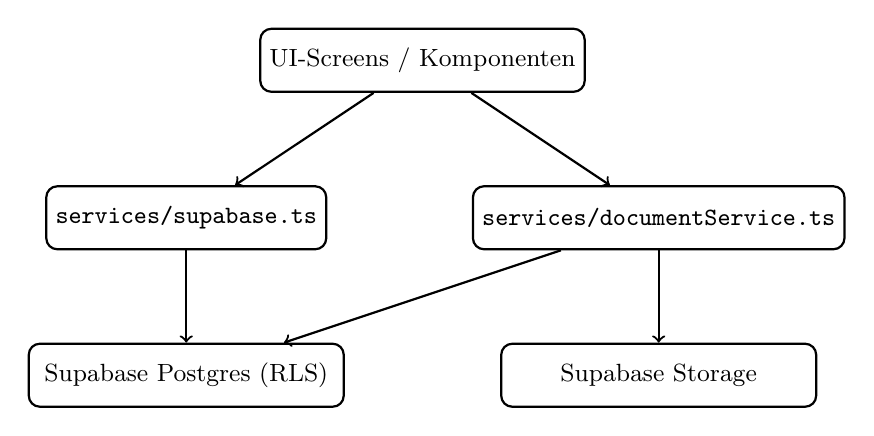
\begin{tikzpicture}[
    x=1cm, y=1cm,
    box/.style={draw, rounded corners, thick, minimum width=4.0cm,
                minimum height=0.8cm, align=center, font=\small},
    thin/.style={draw, rounded corners, thick, minimum width=3.2cm,
                 minimum height=0.8cm, align=center, font=\small\ttfamily},
    arr/.style={->, thick}
  ]
    \node[box]  (ui)      at (0,0)    {UI-Screens / Komponenten};
    \node[thin] (supa)    at (-3,-2)  {services/supabase.ts};
    \node[thin] (docsvc)  at (3,-2)   {services/documentService.ts};
    \node[box]  (db)      at (-3,-4)  {Supabase Postgres (RLS)};
    \node[box]  (storage) at (3,-4)   {Supabase Storage};

    \draw[arr] (ui)     -- (supa);
    \draw[arr] (ui)     -- (docsvc);
    \draw[arr] (supa)   -- (db);
    \draw[arr] (docsvc) -- (storage);
    \draw[arr] (docsvc) -- (db);
  \end{tikzpicture}
  \caption{Service-Layer zwischen UI und Datenhaltung in Skyline}
  \label{fig:service_layer}
\end{figure}

Diese Trennung verfolgt drei Ziele:

\begin{itemize}
  \item \textbf{Single Responsibility:} Jede UI-Komponente ist ausschließlich
        für die Darstellung zuständig und kennt keine Datenbankdetails.
        Änderungen am Schema oder an der Supabase-Abfragelogik erfordern nur
        Anpassungen im Service, nicht in den Screens.
  \item \textbf{Konsistente Fehlerbehandlung:} Rollback-Logik (z.\,B. Löschen
        einer hochgeladenen Datei bei DB-Fehler), Timeout-Fallbacks und
        URL-Refresh-Mechanismen sind zentral im Service implementiert und
        stehen allen Screens zur Verfügung.
  \item \textbf{Testbarkeit:} Der Service-Layer kann isoliert getestet werden,
        ohne dass eine vollständige UI gerendert werden muss.
\end{itemize}

Aus Sicht der Datenverwaltung ist besonders relevant, dass der Service-Layer
die RLS-Grenzen der Datenbank \emph{nicht} umgehen kann und auch nicht soll.
Selbst wenn eine fehlerhafte UI-Komponente eine Abfrage ohne
\texttt{profile\_id}-Filter absetzt, greift die RLS-Policy auf Datenbankebene
und gibt ausschließlich die eigenen Datensätze zurück.
Der Service-Layer ist damit kein Sicherheitsmechanismus, sondern eine
Schicht für Wartbarkeit und Konsistenz -- die eigentliche Sicherheit liegt
in der Datenbank selbst.

% ============================================================
\subsection{Beziehung Flight \texorpdfstring{$\leftrightarrow$}{<->}
            Notes, Docs \& Checklists}
% ============================================================

Die Verknüpfung zwischen Flugstammdaten und Zusatzinformationen erfolgt in Skyline konsistent
über \texttt{flight\_id}.
Sowohl \texttt{user\_notes} als auch \texttt{user\_checklists} und \texttt{flight\_documents}
referenzieren jeweils genau einen Datensatz in \texttt{user\_flights}.

Technisch ist diese Beziehung als Foreign Key mit \texttt{ON DELETE CASCADE} umgesetzt.
Listing~\ref{lst:fk_cascade} zeigt dies exemplarisch für \texttt{flight\_documents}:

\begin{lstlisting}[style=skyline-sql,
  caption={Foreign Key mit ON DELETE CASCADE in \texttt{flight\_documents}
           (migration\_add\_flight\_documents.sql)},
  label={lst:fk_cascade}]
CREATE TABLE IF NOT EXISTS public.flight_documents (
  id         UUID PRIMARY KEY DEFAULT gen_random_uuid(),
  flight_id  UUID NOT NULL
             REFERENCES public.user_flights(id) ON DELETE CASCADE,
  profile_id UUID NOT NULL
             REFERENCES public.profiles(id)     ON DELETE CASCADE,
  file_name  TEXT    NOT NULL,
  file_type  TEXT    NOT NULL
             CHECK (file_type IN ('pdf', 'image', 'other')),
  mime_type  TEXT    NOT NULL,
  file_size  BIGINT  NOT NULL,
  storage_path       TEXT NOT NULL,
  storage_bucket     TEXT NOT NULL DEFAULT 'flight-documents',
  signed_url         TEXT,
  signed_url_expires_at TIMESTAMPTZ,
  document_type TEXT
    CHECK (document_type IN
           ('boarding_pass','booking_confirmation','receipt','other'))
    DEFAULT 'other',
  is_cached  BOOLEAN DEFAULT FALSE,
  cache_path TEXT,
  uploaded_at TIMESTAMPTZ DEFAULT NOW()
);
\end{lstlisting}

Für alle Tabellen sind RLS-Policies definiert, die sicherstellen, dass ein Nutzer
ausschließlich eigene Datensätze lesen und schreiben kann.
Listing~\ref{lst:rls_notes} zeigt die vier Policies für \texttt{user\_notes}:

\begin{lstlisting}[style=skyline-sql,
  caption={Row-Level-Security-Policies für \texttt{user\_notes}
           (complete\_working\_schema.sql)},
  label={lst:rls_notes}]
ALTER TABLE public.user_notes ENABLE ROW LEVEL SECURITY;

CREATE POLICY "notes_select_own" ON public.user_notes
  FOR SELECT USING (profile_id = auth.uid());

CREATE POLICY "notes_insert_own" ON public.user_notes
  FOR INSERT WITH CHECK (profile_id = auth.uid());

CREATE POLICY "notes_update_own" ON public.user_notes
  FOR UPDATE USING (profile_id = auth.uid());

CREATE POLICY "notes_delete_own" ON public.user_notes
  FOR DELETE USING (profile_id = auth.uid());
\end{lstlisting}

% Screenshot RLS-Policy-Übersicht
\begin{figure}[htbp]
  \centering
  \fbox{\parbox{0.88\textwidth}{\centering\vspace{1.2cm}
    \textbf{TODO: Screenshot einfügen}\\[0.3cm]
    Supabase Dashboard $\rightarrow$ Authentication $\rightarrow$ Policies\\
    (RLS-Policy-Liste für Tabelle \texttt{user\_notes} oder \texttt{user\_flights})
    \vspace{1.2cm}}}
  \caption{Row-Level-Security-Policies im Supabase Dashboard}
  \label{fig:supabase_rls}
\end{figure}

In der App-Logik wird die Beziehung ebenfalls explizit genutzt.
Listing~\ref{lst:get_notes} zeigt die Abfrage von Notizen pro Flug in
\texttt{services/supabase.ts}:

\begin{lstlisting}[style=skyline-ts,
  caption={Flugbezogene Notizen-Abfrage mit \texttt{profile\_id}-Filter
           (services/supabase.ts)},
  label={lst:get_notes}]
async getNotes(flightId: string): Promise<Note[]> {
  const user = (await this.supabase.auth.getUser()).data.user;
  if (!user) return [];

  const { data, error } = await this.supabase
    .from('user_notes')
    .select('id, profile_id, flight_id, purpose,
             title, content, reminder_at,
             created_at, updated_at')
    .eq('flight_id', flightId)   // nur dieser Flug
    .eq('profile_id', user.id)   // nur eigene Notizen
    .order('created_at', { ascending: true });

  if (error) throw error;
  return (data || []).map((n): Note => ({ ... }));
}
\end{lstlisting}

Die Detailansicht (\texttt{trip-details.tsx}) stößt beim Öffnen alle abhängigen
Ladevorgänge parallel an:

\begin{lstlisting}[style=skyline-ts,
  caption={Paralleles Vorladen in der Trip-Detailansicht (app/trip-details.tsx)},
  label={lst:parallel_load}]
void Promise.allSettled([
  loadNotesForFlight(id),
  loadChecklistsForFlight(id),
  loadTemplatesByPurpose('private'),
]);
\end{lstlisting}

\begin{figure}[htbp]
  \centering
  \begin{tikzpicture}[
    x=1cm, y=1cm,
    box/.style={draw, rounded corners, thick, minimum width=3.0cm,
                minimum height=0.8cm, align=center, font=\small\ttfamily},
    step/.style={draw, rounded corners, thick, minimum width=3.8cm,
                 minimum height=0.8cm, align=center, font=\small},
    arr/.style={->, thick}
  ]
    \node[step] (open) at (0,0)    {Nutzer öffnet Flug};
    \node[step] (par)  at (0,-1.5) {Promise.allSettled()};
    \node[box]  (n)    at (-3.5,-3){user\_notes};
    \node[box]  (c)    at (0,-3)   {user\_checklists};
    \node[box]  (d)    at (3.5,-3) {flight\_documents};
    \node[step] (ui)   at (0,-4.5) {Detailansicht bereit};
    \draw[arr] (open)--(par);
    \draw[arr] (par)--(n);  \draw[arr] (par)--(c);  \draw[arr] (par)--(d);
    \draw[arr] (n)--(ui);   \draw[arr] (c)--(ui);   \draw[arr] (d)--(ui);
  \end{tikzpicture}
  \caption{Paralleles Laden flugbezogener Daten beim Öffnen der Trip-Detailansicht}
  \label{fig:parallel_load}
\end{figure}

% ============================================================
\subsection{Storage-Bucket \& Signed URLs}
% ============================================================

Dateibasierte Inhalte -- Boardingpässe, Buchungsbestätigungen, Belege -- werden im
Supabase-Storage-Bucket \texttt{flight-documents} abgelegt.
Der Bucket ist privat konfiguriert; öffentlicher Dauerzugriff ist nicht möglich.
Jedes Dokument erhält einen strukturierten Pfad,
der in \texttt{DocumentService.generateStoragePath()} berechnet wird:

\begin{lstlisting}[style=skyline-ts,
  caption={Pfadgenerierung im Storage-Bucket (services/documentService.ts)},
  label={lst:storage_path}]
private generateStoragePath(
  userId: string, flightId: string, fileName: string
): string {
  const timestamp = Date.now();
  const sanitized = fileName.replace(/[^a-zA-Z0-9.-]/g, '_');
  return `${userId}/${flightId}/${timestamp}_${sanitized}`;
}
\end{lstlisting}

Nach dem Upload wird die Signed URL sofort generiert und zusammen mit den Metadaten
in \texttt{flight\_documents} gespeichert.
Listing~\ref{lst:signed_url} zeigt den Upload- und URL-Erzeugungsschritt:

\begin{lstlisting}[style=skyline-ts,
  caption={Upload und Signed-URL-Erzeugung (services/documentService.ts)},
  label={lst:signed_url}]
// Datei hochladen
const { error: uploadError } = await supabase.storage
  .from(this.bucketName)       // 'flight-documents'
  .upload(storagePath, fileData, {
    cacheControl: '3600',
    contentType: mimeType,
    upsert: false,
  });

// Signed URL erzeugen (gueltig: 3600 Sekunden)
const { data: signedUrlData } = await supabase.storage
  .from(this.bucketName)
  .createSignedUrl(storagePath, this.signedUrlExpirationSeconds);

// Metadaten + URL in DB speichern
await supabase.from('flight_documents').insert({
  flight_id:             flightId,
  storage_path:          storagePath,
  signed_url:            signedUrlData?.signedUrl,
  signed_url_expires_at: expiresAt.toISOString(),
  document_type:         documentType,
  ...
});
\end{lstlisting}

Ist eine gespeicherte URL abgelaufen, wird sie in \texttt{getDocumentUrl()} automatisch
erneuert (Listing~\ref{lst:url_refresh}):

\begin{lstlisting}[style=skyline-ts,
  caption={Automatischer Signed-URL-Refresh (services/documentService.ts)},
  label={lst:url_refresh}]
// Pruefen ob URL noch gueltig
if (doc.signed_url && doc.signed_url_expires_at) {
  if (new Date(doc.signed_url_expires_at) > new Date()) {
    return doc.signed_url; // noch gueltig
  }
}

// Neue URL generieren und in DB aktualisieren
const { data: signedUrlData } = await supabase.storage
  .from(this.bucketName)
  .createSignedUrl(doc.storage_path, this.signedUrlExpirationSeconds);

await supabase.from('flight_documents').update({
  signed_url:            signedUrlData.signedUrl,
  signed_url_expires_at: expiresAt.toISOString(),
}).eq('id', documentId);
\end{lstlisting}

% Screenshot Storage-Bucket
\begin{figure}[htbp]
  \centering
  \fbox{\parbox{0.88\textwidth}{\centering\vspace{1.2cm}
    \textbf{TODO: Screenshot einfügen}\\[0.3cm]
    Supabase Dashboard $\rightarrow$ Storage $\rightarrow$ Bucket
    \texttt{flight-documents}\\
    (Ordnerstruktur \texttt{userId/flightId/...} mit hochgeladenen Dateien sichtbar)
    \vspace{1.2cm}}}
  \caption{Storage-Bucket \texttt{flight-documents} im Supabase Dashboard}
  \label{fig:supabase_storage}
\end{figure}

\begin{figure}[htbp]
  \centering
  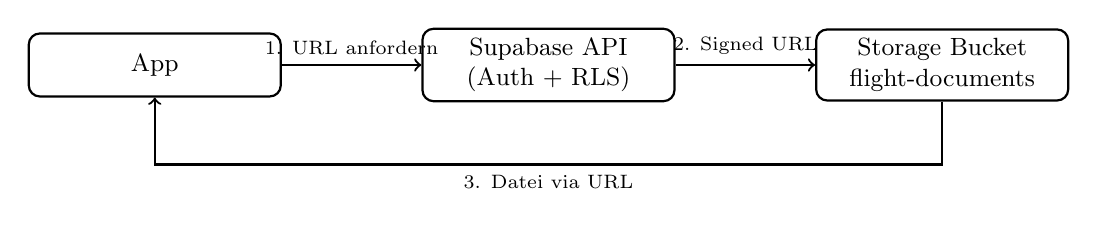
\begin{tikzpicture}[
    x=1cm, y=1cm,
    box/.style={draw, rounded corners, thick, minimum width=3.2cm,
                minimum height=0.8cm, align=center, font=\small},
    arr/.style={->, thick},
    note/.style={font=\scriptsize, align=center}
  ]
    \node[box] (app)     at (0,0)  {App};
    \node[box] (api)     at (5,0)  {Supabase API\\(Auth + RLS)};
    \node[box] (storage) at (10,0) {Storage Bucket\\flight-documents};

    \draw[arr] (app) -- node[above,note]{1. URL anfordern} (api);
    \draw[arr] (api) -- node[above,note]{2. Signed URL} (storage);
    \draw[arr] (storage.south) -- ++(0,-0.8) -|
      node[below,note,pos=0.25]{3. Datei via URL} (app.south);
  \end{tikzpicture}
  \caption{Dokumentenzugriff über Signed URLs in Skyline}
  \label{fig:signed_url_flow}
\end{figure}

% ============================================================
\subsection{Sync-Strategie \& Caching}
% ============================================================

Die Synchronisationsstrategie von Skyline ist auf schnelle Startzeit bei gleichzeitig
konsistentem Online-Datenstand ausgelegt.
Beim App-Start ruft \texttt{\_layout.tsx} zunächst \texttt{loadFlights()} auf.
Anschließend werden für die ersten 12 Flüge Notizen und Checklisten vorab geladen
(\emph{Warmup}), damit die Detailansicht ohne Erstladeverzögerung öffnet:

\begin{lstlisting}[style=skyline-ts,
  caption={Warmup beim App-Start: paralleles Vorladen von Notes und Checklists
           (app/\_layout.tsx)},
  label={lst:warmup}]
const flightIds = useAppStore.getState().flights
  .map(f => f?.id)
  .filter(id => typeof id === 'string')
  .slice(0, 12); // max. 12 Fluege vorladen

const preloadTasks: Promise<any>[] = [];
for (const flightId of flightIds) {
  preloadTasks.push(loadNotesForFlight(flightId));
  preloadTasks.push(loadChecklistsForFlight(flightId));
}
await Promise.allSettled(preloadTasks);
\end{lstlisting}

Dokumente können lokal gecacht werden.
Der Cache-Zustand wird in \texttt{is\_cached} und \texttt{cache\_path} in der Tabelle
\texttt{flight\_documents} mitgeführt.
Beim nächsten Zugriff prüft die App zunächst den lokalen Cache, bevor eine Signed URL
angefordert wird.
Fachliche Kerndaten (Flüge, Notizen, Checklisten) werden primär aus Supabase bezogen;
lokale Caches dienen der Beschleunigung, nicht als unabhängiger Primärspeicher.

% ============================================================
\subsection{Fehlerfälle \& Wiederherstellung}
% ============================================================

Die Implementierung enthält mehrere Schutzmechanismen, um Fehlerfälle ohne Datenverlust
und ohne instabile UI-Zustände zu behandeln.

\textbf{Storage-Rollback beim Upload:}
Schlägt nach erfolgreichem Storage-Upload die Metadatenpersistierung in der Datenbank fehl,
löscht \texttt{DocumentService} die bereits hochgeladene Datei wieder:

\begin{lstlisting}[style=skyline-ts,
  caption={Storage-Rollback bei DB-Fehler (services/documentService.ts)},
  label={lst:rollback}]
if (dbError) {
  // Cleanup: hochgeladene Datei entfernen,
  // damit kein Datei-Eintrag ohne DB-Referenz bleibt
  await supabase.storage
    .from(this.bucketName)
    .remove([storagePath]);
  throw new Error(
    `Failed to save document metadata: ${dbError.message}`
  );
}
\end{lstlisting}

\textbf{Cache-Invalidierung:}
Ist ein als lokal markiertes Dokument nicht mehr am erwarteten Pfad vorhanden,
wird der Cache-Status in den Metadaten zurückgesetzt:

\begin{lstlisting}[style=skyline-ts,
  caption={Cache-Validierung und -Reset (services/documentService.ts)},
  label={lst:cache_invalidate}]
const fileInfo = await FileSystem.getInfoAsync(doc.cache_path);
if (!fileInfo.exists) {
  // Cache ungueltig -> in DB zuruecksetzen
  await supabase.from('flight_documents').update({
    is_cached: false,
    cache_path: null,
  }).eq('id', documentId);
  return null; // App laedt anschliessend aus Online-Bestand
}
\end{lstlisting}

\textbf{UI-Timeout in der Dokumentliste:}
\texttt{DocumentList.tsx} setzt einen 10-Sekunden-Timeout, um Endlosschleifen bei
Ladeindikatoren zu verhindern:

\begin{lstlisting}[style=skyline-ts,
  caption={Timeout-Fallback beim Laden der Dokumentliste
           (components/documents/DocumentList.tsx)},
  label={lst:timeout}]
// 10-Sekunden-Timeout verhindert haengenden Ladeindikator
timeoutId = setTimeout(() => {
  if (isMountedRef.current) {
    setLoading(false);
    setDocuments([]); // Fallback: leere Liste statt Endlosschleifen
  }
}, 10000);

const docs = await documentService.getDocumentsForFlight(flightId);
clearTimeout(timeoutId);
setDocuments(docs || []);
\end{lstlisting}

% ============================================================
\section{Bewertung der Wirkung}
% ============================================================

Die in Kapitel~5.1 beschriebene Implementierung wird in diesem Abschnitt dahingehend
bewertet, ob die gesetzten Ziele -- erhöhte Transparenz und verbesserte
Nachvollziehbarkeit -- durch die gewählte Datenverwaltungsarchitektur tatsächlich
erreicht werden.
Als Vergleichsmaßstab dient die typische dezentrale Ablagesituation, bei der
Buchungsbestätigungen in E-Mails, Dokumente in der Foto-App und Reisenotizen in
separaten Tools verwaltet werden.

% ------------------------------------------------------------
\subsection{KPI: Transparenz}
% ------------------------------------------------------------

Als primärer KPI für Transparenz wurde definiert: die Zeit, die ein Nutzer benötigt,
um den vollständigen Status einer Reise zu erfassen -- also ob Dokumente vorhanden sind,
welche Checklisten noch offen stehen und wann der nächste Flug stattfindet.

Durch die zentrale Verknüpfung aller Daten über \texttt{flight\_id} öffnet die
Trip-Detailansicht alle relevanten Informationen auf einem einzigen Screen.
Dabei werden Notizen, Checklisten und Dokumente beim Öffnen parallel vorgeladen
(\texttt{Promise.allSettled}), sodass keine sequentiellen Ladezeiten entstehen.
Ein Warmup-Mechanismus beim App-Start lädt die ersten zwölf Flüge bereits im
Hintergrund, was die wahrgenommene Reaktionszeit weiter reduziert.

Das Feld \texttt{status} in \texttt{user\_flights} (\texttt{upcoming}/
\texttt{completed}/\texttt{cancelled}) erlaubt eine sofortige Einschätzung
des Reisestatus ohne Öffnen der Detailansicht.
Die Felder \texttt{departure\_at} und \texttt{arrival\_at} ermöglichen darüber
hinaus eine Live-Fortschrittsanzeige auf der Karte sowie zeitbasierte
Erinnerungen -- beides Funktionen, die bei verteilter Datenhaltung nicht
umsetzbar wären, da die notwendigen Zeitdaten fehlen oder inkonsistent verteilt wären.

% ------------------------------------------------------------
\subsection{KPI: Nachvollziehbarkeit}
% ------------------------------------------------------------

Als zweiter KPI wurde die Zeit bis zum Wiederfinden eines bestimmten Dokuments
oder Belegs definiert -- ein im Geschäftsreisekontext besonders relevanter Aspekt,
etwa bei der Reisekostenabrechnung.

Die Kategorisierung über \texttt{document\_type} (\texttt{boarding\_pass},
\texttt{booking\_confirmation}, \texttt{receipt}, \texttt{other}) ermöglicht
eine strukturierte, filterbare Dokumentliste direkt im Flugkontext.
Im Gegensatz zu einer E-Mail-Suche oder einem Foto-App-Scroll entfällt jedes
manuelle Sortieren: Jeder Beleg ist genau dem Flug zugeordnet, zu dem er gehört.

Zusätzlich trägt jede Entität im Datenmodell Zeitstempel (\texttt{created\_at},
\texttt{updated\_at}), die eine lückenlose zeitliche Rückverfolgbarkeit ermöglichen.
Die Foreign-Key-Kette \texttt{profile\_id $\to$ user\_flights $\to$ flight\_documents}
stellt sicher, dass jeder Datensatz eindeutig einem Nutzer und einem Flug zugeordnet
werden kann -- auch rückwirkend, z.\,B. für Auditingzwecke im Firmenkontext.

% ------------------------------------------------------------
\subsection{Vergleich zu dezentralen Lösungen}
% ------------------------------------------------------------

Ohne zentrale Datenverwaltung ist die Informationslage bei Geschäftsreisen
typischerweise stark fragmentiert: Buchungsbestätigungen liegen als E-Mails vor,
Boardingpässe in der Wallet-App, Quittungen als Fotos, Notizen in einem separaten
Notiztool.
Dieses Szenario erzeugt mehrere konkrete Probleme:

\begin{itemize}
  \item \textbf{Suchaufwand:} Das Wiederfinden eines Belegs erfordert das Durchsuchen
        mehrerer Apps und Postfächer.
  \item \textbf{Inkonsistenz:} Daten können veraltet oder in einer der Quellen gelöscht
        sein, ohne dass dies in anderen Apps sichtbar wird.
  \item \textbf{Fehlende Verknüpfung:} Ein Flug ohne zugehörige Dokumente ist nicht
        als unvollständig erkennbar -- der Nutzer muss manuell prüfen.
  \item \textbf{Sicherheit:} Dokumente in der Foto-App oder in E-Mail-Anhängen sind
        nicht zugriffsgeschützt; jeder mit Gerätezugriff kann sie einsehen.
\end{itemize}

Skyline eliminiert diese Fragmentierung durch das Single-Source-of-Truth-Prinzip:
Alle reisebezogenen Daten sind in einem konsistenten, relational verknüpften Modell
gespeichert.
RLS stellt dabei sicher, dass selbst bei Datenbankzugriff außerhalb der App
kein Nutzer auf Daten eines anderen zugreifen kann.
Für den Teamkontext gilt zusätzlich das Prinzip der minimalen Sichtbarkeit:
Mitglieder einer Firma sehen nur Profile derselben Company -- nicht das
gesamte Nutzerverzeichnis.

% ============================================================
\section{Ergebnis}
% ============================================================

Die implementierte zentrale Datenverwaltung erfüllt die in Kapitel~3 formulierten
Anforderungen an Transparenz und Nachvollziehbarkeit.
Das gewählte Architekturmuster -- Single Source of Truth auf Basis von
Supabase Postgres, ergänzt durch Supabase Storage für Binärdaten -- hat sich
als tragfähig erwiesen und skaliert sowohl für Einzelnutzer als auch für
den Teamkontext.

% ------------------------------------------------------------
\subsection{Verbesserungen in Transparenz}
% ------------------------------------------------------------

Durch die flugzentrierte Datenstruktur sind Status, Dokumente, Notizen und
Checklisten jederzeit kontextbezogen abrufbar.
Der Nutzer muss keine mehreren Apps oder Postfächer durchsuchen; alle
reiserelevanten Informationen sind auf einem einzigen Screen zusammengefasst.
Zeitfelder (\texttt{departure\_at}, \texttt{arrival\_at}) ermöglichen eine
Echtzeit-Fortschrittsanzeige, die bei dezentraler Datenhaltung strukturell
nicht realisierbar wäre.
RLS stellt sicher, dass diese Transparenz auf die eigenen Daten beschränkt
bleibt -- kein Nutzer sieht unbeabsichtigt Daten eines anderen.

% ------------------------------------------------------------
\subsection{Verbesserungen in Nachvollziehbarkeit}
% ------------------------------------------------------------

Die kategorisierte Dokumentablage (\texttt{document\_type}) und die
\texttt{flight\_id}-Verknüpfung reduzieren den Aufwand beim Wiederfinden
eines Belegs auf einen gezielten Filter -- anstelle einer systemübergreifenden Suche.
Alle Entitäten tragen \texttt{created\_at} und \texttt{updated\_at},
sodass Änderungshistorien nachvollziehbar bleiben.
Die Foreign-Key-Kette vom Profil über den Flug zu jedem Dokument
ermöglicht eine vollständige Rückverfolgbarkeit jedes Reisedatensatzes,
was insbesondere für Reisekostenabrechnungen und Compliance-Anforderungen
im Firmenkontext relevant ist.

% ------------------------------------------------------------
\subsection{Schlussfolgerung}
% ------------------------------------------------------------

Die Kombination aus Single Source of Truth, Security-by-Design (RLS,
private Storage-Buckets, zeitlich begrenzte Signed URLs) und einem
robusten Fehlerbehandlungskonzept (Storage-Rollback bei DB-Fehler,
automatischer URL-Refresh, Cache-Invalidierung) liefert ein nachhaltiges
und erweiterungsfähiges Datenfundament für Skyline.

Bestehende Schwachstellen dezentraler Lösungen -- Fragmentierung,
fehlende Verknüpfung, mangelnder Zugriffsschutz -- werden durch die
gewählte Architektur strukturell adressiert, nicht nur kompensiert.
Das migrationsbasierte Vorgehensmodell stellt dabei sicher, dass das
Schema auch in zukünftigen Entwicklungsiterationen ohne Datenverlust
erweitert werden kann.

%!TEX root = ../DA_MainDocument.tex

% ============================================================
\section{Rechtliche Rahmenbedingungen (projektrelevant)}\label{sec:recht}
% ============================================================

Die Skyline-App verarbeitet personenbezogene Daten in mehreren funktionalen
Bereichen: Benutzerprofile, Flug- und Reisedaten, Notizen, Checklisten sowie
hochgeladene Reisedokumente.
Rechtsdogmatisch handelt es sich um eine automatisierte Verarbeitung
personenbezogener Daten im Sinne des Art.~4 Z~1 und Z~2 DSGVO
\cite{gdpr}, da Informationen verarbeitet werden, die sich auf identifizierte
oder identifizierbare natürliche Personen beziehen.
Der Anwendungsbereich der Datenschutz-Grundverordnung ist damit gemäß
Art.~2 Abs.~1 DSGVO vollständig eröffnet.

Da Skyline auf Supabase als Backend-Plattform aufsetzt, werden Authentifizierung,
Datenbankzugriff und Dateispeicherung technisch zentral über eine
cloudbasierte Infrastruktur verwaltet \cite{supabasePlatform}.
Diese Architektur ermöglicht die Umsetzung datenschutzrechtlicher Anforderungen
auf mehreren Ebenen gleichzeitig: sichere Authentifizierung, datenbankbasierte
Zugriffskontrolle über Row-Level Security sowie kontrollierter Dateizugriff
über zeitlich begrenzte Signed URLs.

% ============================================================
\subsection{Datenschutzrechtliche Vorgaben (DSGVO)}
% ============================================================

Die DSGVO \cite{gdpr} bildet den primären Rechtsrahmen für die Verarbeitung
personenbezogener Daten innerhalb von Skyline.
Ergänzend gilt das österreichische Datenschutzgesetz (DSG) \cite{dsg},
das nationale Präzisierungen und Öffnungsklauseln zur DSGVO enthält.
Maßgeblich sind insbesondere die Grundsätze aus Art.~5 DSGVO:
Rechtmäßigkeit, Zweckbindung, Datenminimierung, Richtigkeit,
Speicherbegrenzung sowie Integrität und Vertraulichkeit.

Für Skyline sind vor allem die Grundsätze der Zweckbindung,
der Datenminimierung sowie der Integrität und Vertraulichkeit
technisch umzusetzen.
Reiseprofile können, auch ohne besondere Kategorien im Sinne des Art.~9 DSGVO
zu berühren, durch die Kombination von Bewegungsdaten, Aufenthaltsorten
und beruflichen Kontexten ein erhöhtes Schutzbedürfnis begründen.
Die Systemarchitektur muss daher sicherstellen, dass unbefugte Zugriffe
strukturell -- und nicht nur durch App-seitige Filter -- ausgeschlossen sind.

% ------------------------------------------------------------
\subsubsection{Speicherung und Verarbeitung personenbezogener Daten}
% ------------------------------------------------------------

In Skyline werden die folgenden Kategorien personenbezogener Daten verarbeitet:

\begin{itemize}
  \item \textbf{Stammdaten:} Name, E-Mail-Adresse (via Supabase Auth),
        optional Profilbild (\texttt{avatar\_url}), Kontotyp
        (\texttt{account\_type}: \texttt{worker}/\texttt{company}),
        nutzerspezifische Einstellungen (\texttt{preferences}, JSONB).

  \item \textbf{Reise- und Flugdaten:} Flugnummer, Airline, Datum,
        Abflug- und Ankunftszeiten (\texttt{departure\_at},
        \texttt{arrival\_at}), Gate, Terminal, Sitzplatznummer,
        Buchungsbestätigungscode, Buchungsreferenz (PNR),
        Flugstatus sowie die berechnete Flugdistanz.
        Diese Felder werden in der Tabelle \texttt{user\_flights}
        flugbezogen gespeichert.

  \item \textbf{Inhalts- und Kommunikationsdaten:} Freitextnotizen
        (\texttt{user\_notes}), Checklisten mit Einzelpunkten
        (\texttt{user\_checklists}, \texttt{user\_checklist\_items})
        sowie ein optionales Erinnerungsfeld (\texttt{reminder\_at}).

  \item \textbf{Dokumentendaten:} Dateiname, MIME-Type, Dateigröße,
        Storage-Pfad sowie der Dateiinhalt selbst (im privaten
        Storage-Bucket \texttt{flight-documents}).
        Metadaten werden in der Tabelle \texttt{flight\_documents}
        verwaltet; der Kategorie-Typ (\texttt{document\_type}) erlaubt
        eine strukturierte Unterscheidung zwischen Boardingpässen,
        Buchungsbestätigungen, Quittungen und sonstigen Dokumenten.
\end{itemize}

Die Verarbeitung erfolgt zweckgebunden im Sinne des Art.~5 Abs.~1
lit.~b DSGVO zur Organisation und Verwaltung von Flugreisen.
Die Datenbankstruktur unterstützt diese Zweckbindung unmittelbar:
Alle Zusatzinformationen (Notizen, Dokumente, Checklisten) sind über
einen Foreign Key mit \texttt{ON DELETE CASCADE} an genau einen
Flugkontext gebunden -- eine Verwahrung losgelöster Datensätze ist
strukturell ausgeschlossen.

Im Teamkontext basiert der Datenzugriff auf einer kontrollierten
Zuordnung über \texttt{company\_id} und \texttt{company\_members}.
Ohne Mitgliedschaft in einer Firma ist kein Zugriff auf Firmendaten
möglich; das Prinzip der Zugriffsbeschränkung ist damit technisch
erzwungen, nicht nur konzeptionell formuliert.

% ------------------------------------------------------------
\subsubsection{Maßnahmen zur sicheren Datenverarbeitung}
% ------------------------------------------------------------

Gemäß Art.~32 DSGVO sind geeignete technische und organisatorische
Maßnahmen (TOM) umzusetzen, um ein dem Risiko angemessenes Schutzniveau
zu gewährleisten \cite{edpbArt32}.
In Skyline werden die folgenden technischen Maßnahmen implementiert:

\begin{description}
  \item[Authentifizierung über Supabase Auth \cite{supabaseAuth}:]
    Zugriff auf personenbezogene Daten ist ausschließlich nach
    erfolgreicher Authentifizierung möglich.
    Die Benutzer-ID (\texttt{auth.uid()}) bildet die Grundlage aller
    datenbankinternen Zugriffskontrollen.
    Login-, Signup- und Passwort-Reset-Prozesse sind vollständig
    über Supabase Auth abgewickelt; Passwörter werden nicht im
    Klartext gespeichert.

  \item[Row-Level Security (RLS) \cite{supabaseRLS}:]
    Alle operativen Tabellen (\texttt{user\_flights},
    \texttt{user\_notes}, \texttt{user\_checklists},
    \texttt{user\_checklist\_items}, \texttt{flight\_documents} u.\,a.)
    sind durch RLS-Policies geschützt.
    Abfragen werden datenbanksseitig auf die eigenen Datensätze
    des authentifizierten Nutzers eingeschränkt.
    Selbst fehlerhafte oder böswillige Anfragen ohne clientseitigen
    Filter können nicht auf fremde Daten zugreifen.
    Die Policies folgen dem Muster
    \texttt{USING (profile\_id = auth.uid())} für Lese-,
    Änderungs- und Löschoperationen sowie
    \texttt{WITH CHECK (profile\_id = auth.uid())} für Schreiboperationen.

  \item[Private Storage-Buckets \cite{supabaseStorage}:]
    Dokumente werden im privaten Supabase-Storage-Bucket
    \texttt{flight-documents} abgelegt.
    Kein dauerhafter öffentlicher Direktzugriff ist möglich;
    der Bucket erfordert eine aktive Zugriffskontrolle für
    jeden Dateiaufruf.

  \item[Signed URLs mit begrenzter Gültigkeit:]
    Dateizugriffe erfolgen über zeitlich limitierte,
    signierte URLs (Gültigkeitsdauer: 3.600 Sekunden).
    Abgelaufene URLs werden vom \texttt{DocumentService}
    automatisch erneuert und in der Datenbank aktualisiert.
    Dauerhaft gültige Direktlinks auf Dokumente sind
    architektonisch ausgeschlossen.

  \item[Transportverschlüsselung:]
    Die gesamte Kommunikation zwischen App und Supabase-Backend
    erfolgt über HTTPS/TLS.
    Vertraulichkeit und Integrität der Daten sind während
    des Transports gewährleistet.

  \item[Strukturierte Speicherpfade:]
    Dokumente im Storage-Bucket werden nach dem Schema
    \texttt{\{userId\}/\{flightId\}/\{timestamp\}\_\{fileName\}}
    abgelegt.
    Dadurch ist die Eigentümerzuordnung auch auf Dateisystemebene
    eindeutig; zufällige Namenskollisionen werden durch den
    Zeitstempel verhindert.

  \item[Referenzielle Integrität und Datenlebenszyklus:]
    Foreign Keys mit \texttt{ON DELETE CASCADE} stellen sicher,
    dass beim Löschen eines Nutzerprofils oder eines Fluges
    alle verknüpften Daten (Notizen, Checklisten, Dokumente)
    automatisch mitgelöscht werden.
    Verwaiste Datensätze ohne zugehörigen Kontext entstehen
    strukturell nicht.
    Dies unterstützt die Speicherbegrenzung im Sinne des
    Art.~5 Abs.~1 lit.~e DSGVO.

  \item[Transaktionaler Rollback bei Upload-Fehlern:]
    Schlägt nach einem erfolgreichen Storage-Upload das
    Schreiben der Metadaten in die Datenbank fehl,
    löscht der \texttt{DocumentService} die hochgeladene
    Datei automatisch wieder.
    Es entstehen keine unbeschrifteten Dateien im Bucket,
    denen kein Datenbankdatensatz gegenübersteht.
\end{description}

% ------------------------------------------------------------
\subsubsection{Rechte der betroffenen Personen}
% ------------------------------------------------------------

Die DSGVO gewährt betroffenen Personen umfangreiche Rechte,
die technisch umzusetzen sind \cite{dsb}:

\begin{itemize}
  \item \textbf{Auskunftsrecht (Art.~15 DSGVO):}
        Skyline speichert alle nutzerbezogenen Daten strukturiert
        in verknüpften Tabellen; eine vollständige Datenauskunft
        kann über die \texttt{profile\_id} als Einstiegspunkt
        automatisiert erstellt werden.

  \item \textbf{Recht auf Berichtigung (Art.~16 DSGVO):}
        Profildaten (\texttt{full\_name}, \texttt{avatar\_url},
        \texttt{preferences}), Flugdaten und Notizen sind
        über die App editierbar.
        RLS stellt sicher, dass ein Nutzer nur eigene Daten
        ändern kann.

  \item \textbf{Recht auf Löschung (Art.~17 DSGVO):}
        Durch \texttt{ON DELETE CASCADE} bewirkt das Löschen
        des Nutzerprofils die vollständige Kaskadenlöschung
        aller verknüpften Datensätze.
        Storage-Objekte werden zusätzlich explizit gelöscht,
        da Storage und Datenbank getrennte Systeme sind.

  \item \textbf{Recht auf Einschränkung der Verarbeitung
        (Art.~18 DSGVO) und Datenübertragbarkeit (Art.~20 DSGVO):}
        Die strukturierte, relationale Datenhaltung bildet die
        technische Grundlage für einen Export im maschinenlesbaren
        Format.
\end{itemize}

% ============================================================
\subsection{Datenschutz in Skyline}
% ============================================================

Datenschutz wird in Skyline als architektonisches Prinzip umgesetzt
(\emph{Privacy by Design} gemäß Art.~25 DSGVO \cite{edpbArt25}).
Zugriffskontrollen werden nicht ausschließlich auf Ebene der
Benutzeroberfläche implementiert, sondern primär über
serverseitige Datenbankrichtlinien erzwungen.
Damit entspricht die Implementierung dem Grundsatz
\emph{Privacy by Default}: Standardmäßig sind alle Daten
auf den eigenen Nutzerkontext beschränkt -- eine explizite
Freigabe ist erforderlich, um Daten für andere sichtbar zu machen.

% ------------------------------------------------------------
\subsubsection{Authentifizierung und Zugriffsschutz}
% ------------------------------------------------------------

Der Zugriff auf personenbezogene Daten ist in Skyline ausschließlich
für authentifizierte Benutzer möglich \cite{supabaseAuth}.
Nicht authentifizierte Anfragen können auf keine der durch RLS
geschützten Tabellen zugreifen; der einzige öffentlich zugängliche
Bereich ist die Flughafenstammdatenbank (\texttt{airports}),
die keine personenbezogenen Daten enthält.

Supabase Auth stellt JSON Web Tokens (JWT) aus \cite{rfc7519},
die bei jeder Datenbankoperation serverseitig validiert werden.
Der darin enthaltene Wert \texttt{auth.uid()} entspricht der
\texttt{profile\_id} in allen Nutzertabellen und bildet die
einzige Grundlage für RLS-Entscheidungen.

Im Teamkontext werden zusätzlich Rollen (\texttt{owner},
\texttt{worker}) aus der Tabelle \texttt{company\_members}
berücksichtigt.
Firmeninhaber können Einladungslinks generieren
(\texttt{company\_invites}); erst nach Annahme der Einladung
entsteht ein \texttt{company\_members}-Eintrag, der den
erweiterten Datenzugriff freischaltet.

% ------------------------------------------------------------
\subsubsection{RLS-Policies in Supabase}
% ------------------------------------------------------------

Die zentrale Zugriffskontrolle in Skyline erfolgt über
Row-Level Security-Policies auf PostgreSQL-Ebene \cite{supabaseRLS}.
Tabelle~\ref{tab:rls_uebersicht} gibt eine Übersicht der
Policy-Logik für die wichtigsten Tabellen:

\begin{table}[htbp]
  \centering
  \caption{Übersicht der RLS-Policy-Logik in Skyline}
  \label{tab:rls_uebersicht}
  \begin{tabularx}{\textwidth}{l X}
    \toprule
    \textbf{Tabelle} & \textbf{Policy-Logik (vereinfacht)} \\
    \midrule
    \texttt{profiles}
      & Eigenes Profil: \texttt{id = auth.uid()} \\
      & Firmenmitglieder: EXISTS-Abfrage gegen \texttt{company\_members}
        (gleiche \texttt{company\_id}) \\
    \texttt{user\_flights}
      & \texttt{profile\_id = auth.uid()} für alle Operationen \\
    \texttt{user\_notes}
      & \texttt{profile\_id = auth.uid()} für alle Operationen \\
    \texttt{user\_checklists}
      & \texttt{profile\_id = auth.uid()} für alle Operationen \\
    \texttt{user\_checklist\_items}
      & Indirekt via \texttt{user\_checklists}: EXISTS-Abfrage,
        ob die übergeordnete Checkliste dem Nutzer gehört \\
    \texttt{flight\_documents}
      & \texttt{profile\_id = auth.uid()} für alle Operationen \\
    \texttt{airports}
      & Öffentlich lesbar (\texttt{anon} und \texttt{authenticated});
        kein Personenbezug \\
    \texttt{achievements}
      & Öffentlich lesbar; keine personenbezogenen Daten \\
    \texttt{notifications}
      & \texttt{user\_id = auth.uid()} für alle Operationen \\
    \bottomrule
  \end{tabularx}
\end{table}

Die serverseitige Durchsetzung dieser Policies reduziert das Risiko,
dass fehlerhafte oder manipulierte Client-Abfragen zu unbefugtem
Datenzugriff führen.
Damit wird das Prinzip der Integrität und Vertraulichkeit nach
Art.~5 Abs.~1 lit.~f DSGVO auf technischer Ebene abgesichert --
in Übereinstimmung mit den Empfehlungen der
OWASP Mobile Top 10 \cite{owaspMobileTop10},
die serverseitige Autorisierungsprüfung als kritische Anforderung
für mobile Applikationen ausweisen.

% ------------------------------------------------------------
\subsubsection{Dokumentenspeicherung und Dateirechte}
% ------------------------------------------------------------

Dokumente werden im privaten Supabase-Storage-Bucket
\texttt{flight-documents} gespeichert \cite{supabaseStorage}.
Metadaten (Dateiname, Typ, Größe, Storage-Pfad, Gültigkeitsdauer
der Signed URL) werden in der Tabelle \texttt{flight\_documents}
verwaltet.
Diese Trennung von Metadaten und Binärdaten ermöglicht eine
effiziente Listendarstellung ohne vollständige Dateiübertragung.

Für den Dateizugriff werden ausschließlich zeitlich begrenzte
Signed URLs verwendet.
Öffentliche Permanentlinks auf Nutzer-Dokumente sind
architektonisch ausgeschlossen.
Abgelaufene URLs werden serverseitig automatisch erneuert
und in der Datenbank aktualisiert, sodass die App stets
valide Zugriffslinks vorhält.

Löschvorgänge umfassen sowohl das Storage-Objekt als auch
den zugehörigen Metadateneintrag in der Datenbank.
Durch den transaktionalen Rollback-Mechanismus im
\texttt{DocumentService} wird zudem sichergestellt,
dass keine Dateien im Bucket verbleiben, die keinem
Datenbankdatensatz mehr zugeordnet sind -- ein zentraler
Beitrag zur Speicherbegrenzung im Sinne der DSGVO.

Das Telekommunikationsgesetz 2021 (TKG 2021) \cite{tkg2021}
ist im Kontext der Benachrichtigungs- und Erinnerungsfunktionen
von Skyline relevant, da die App lokale Push-Benachrichtigungen
über den Notification-Service ausliefert.
Die Speicherung von \texttt{fire\_at}, \texttt{kind} und
\texttt{payload} in der Tabelle \texttt{notifications} erfolgt
ausschließlich nutzerbezogen und RLS-gesichert.

